\section{Carla}\cite{carla}
La ricerca per lo sviluppo della guida autonoma in ambiente urbano è  ostacolato da costi infrastrutturali e dalle difficoltà logistiche. È
estremamente difficile avere anche solo un veicolo(che sarebbe comunque insufficiente) a disposizione per il testing e la validazione. Inoltre
alcuni scenari di system verification sono troppo pericolosi per essere eseguiti nel mondo reale. Si pensi ad esempio allo scenario in cui
un pedone attraversa improvvisamente la strada davanti alla macchina. Per questi motivi il training e la validazione vengono spesso fatti in ambiente simulato.  Un simulatore molto adatto a questo scopo, e quello che è stato utilizzato in questo lavoro
è \textbf{Carla}. Carla è un simulatore open source per la guida in ambiente urbano. È stato interamente sviluppato per supportare l'addestramento, la prototipazione
e la validzione di modelli di guida autonoma, includendo percezione e controllo. Carla è una piattaforma libera. Tutti i modelli sono stati creati da zero
e sono liberamente accessibili. Include diversi tipi di layout urbani, di modelli per veicoli,edifici,pedoni,segnali stradali ecc.
La simulazione supporta una moltitudine di sensori differenti e possono essere specificate un ampio numero di condizioni ambientali.
\begin{figure}[h]
    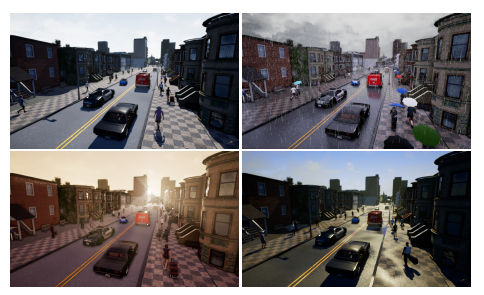
\includegraphics[width = \linewidth]{weather.png}
    \caption{Alcune delle condizioni metereologiche disponibili in Carla}
    \label{fig:weath}
\end{figure}

\subsection{Il motore della simulazione}
L'engine interno è sviluppato sulla base dell'Unreal Engine 4(UE4). Fornisce una fisica reale, npc che seguono una logica elementare e un'ottima qualita di rendering.
Il simulatore provvede una semplice interfaccia tra il mondo e un agente che interagisce con esso. Questa funzionalità è implementata con un'architettura server-client.
Il server esegue la simulazione e il rendering. Il client comunica con il server attraverso un'API implementata in python. L'API permette l'interazione tra l'agente autonomo e il server
attraverso i socket. Il client invia comandi e meta comandi e riceve dati dai sensori. I comandi sono sterzo, accelerazione e frenata. I meta comandi sono usati per modificare le proprietà
del mondo(es. per generare veicoli e pedoni).
\subsection{L'ambiente}
L'ambiente è composto da modelli 3d statici(edifici, vegetazione, segnali stradali, infrastruttre) e modelli dinamici(veicoli, pedoni.). Le dimensioni 
dei modelli sono quanto più possibile realistiche.  Il comportamento degli NPC è stato implementato per mantenere un alto livello di realismo. I veicoli non controllabili
sono basati sul modello standard di UE4(PhysXVehicles). I pedoni si muovono nelle strade seguendo seguendo una mappa di navigazione specifica. Sono incoraggiati a muoversi nei 
marciapiedi e sulle strisce pedonali ma possono attraversare la strada in qualsiasi istante. Per quanto riguarda illuminazione e condizioni atmosferiche si può scegliere tra 18 diverse combinazioni.
Le combinazioni sono date da due possibili condizioni di luminosità(mezzogiorno e tramonto) e nove condizioni metereoligiche. Quest'ultime differiscono per copertura del cielo,
livello di precipitazioni e la presenza o meno di pozze sull'asfalto.
\subsection{Sensori}
I sensori presenti in carla attualmente sono camere RGB e pseudo sensori che forniscono ground truth depth e ground truth semantic segmentation.
Quest'ultimo riconosce 12 categorie semantiche:strada, delimitatore di corsia, segnale stradale, marciapiede, recinzione, palo, muro, edificio, vegetazione
veicolo, pedone e altro.
\begin{figure}[h]
    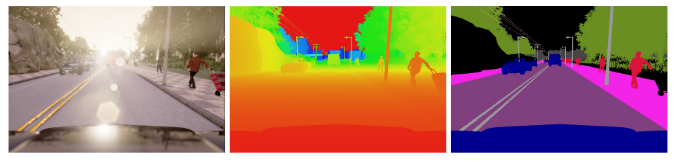
\includegraphics[width = \linewidth]{carlasense.png}
    \caption{Alcuni sensori disponibili:}
    \label{fig:sense}
\end{figure}
In aggiunta alle misure sensoriali, CARLA provvede anche una serie di misure associate allo stato dell'agente e al rispetto delle regole stradali. Le misure 
sullo stato dell'agente riguardano posizione e orientamento del veicolo, velocità, accelerazione, e danni accumulati da collisioni. Per quanto riguarda le regole
stradali vengono riportati stato dei semafori e limite di velocità nella posizione attuale della macchina.
\subsection{Guida Autonoma in CARLA}
CARLA supporta lo sviluppo, l'addestramento e l'analisi delle prestazioni di sistemi di guida autonoma.
Attualmente il simulatore è stato usato per valutare tre approcci:
\begin{itemize}
    \item Modular pipeline
    \item Imitation Learning
    \item Reinforcement Learning
\end{itemize}
Con tutti gli approcci l'agente interagisce con l'ambiente in passi temporali discreti. Ad ogni istante  l'agente riceve un'osservazione O e produce un'azione 
A. L'azione è un vettore tridimensionale che rappresenta lo sterzo, l'accelerazione e il freno. L'osservazione O è formata da una tupla di input
sensoriali monodimensionali(velocità), bidimensionali(GPS) e multidimensionali(immagini rgb, mappe di profondità). Inoltre in tutti gli approcci viene usato
anche un trafitto definito da un planner topologico di alto livello.

\subsubsection{Modular Pipeline}
La guida in tre sottosistemi:
\begin{itemize}
    \item perception
    \item planning
    \item continous control
\end{itemize}

\paragraph{Perception} Per la percezione viene usata una rete di segmentazione semantica basata su RefineNet. La rete viene addestrata per classificare ogni
pixel di un'immagine in una delle seguenti categorie:
\begin{itemize}
    \item strada
    \item marciapiede
    \item delineatore di corsia
    \item oggetto dinamico
    \item oggetto statico
\end{itemize}
Il training set è composto da 2500 immagini etichettate prodotte direttamente all'interno del simultatore
Viene inoltre usato un classificatore binario addestrato su 500 immagini per misurare la probabilità di trovarsi a un incrocio.
\paragraph{planning} Il local planner controlla la navigazione di basso livello generando un insieme di waypoints: punti che rappresentano la posizione e l'orientamento desiderati
negli istanti successivi. Il pianificatore è implementato come una macchina a stati. Gli stati possibili sono:
\begin{itemize}
    \item seguire la strada
    \item girare a sinistra
    \item girare a destra
    \item incrocio
    \item arresto di emergenza
\end{itemize}
Le transizioni avvengono sulla base dei dati raccolti dal modulo di percezioni e dalle informazioni topologiche generate dal global planner.
\paragraph{continous control} controlla gli attuatori per eseguire l'azione voluta. Viene utilizzato un controller PID(proportional-integral-derivative).
Ciascun controller riceve posizione, velocità e lista di waypoints e compie sterzata, accelerazione o frenata.
\subsubsection{Imitation Learning}
Vengono utilizzati dei tragitti registrati di guidatori umani nella città di addestramento. Il dataset è composto da tuple formate da osservazione, azione e comando.
I comandi vengono forniti dai guidatori durante la fase di data collectioni. Sono stati usati 4 comandi: segui la strada, vai dritto al prossimo incrocio, vai a destra al prossimo incrocio e vai a sinistra al 
prossimo incrocio. Le osservazione sono immagini raccolte dalla camera anteriore. E stata aggiunta una perturbazione nel dataset per rendere più robusto il learning.
Il dataset è usato per addestrare un DNN per prevedere l'azione dell'esperto data l'osservazione e il comando.
\subsubsection{Reinforcement Learning}
Una rete viene addestrata sulla base  di un segnale di ricompensa, senza utilizzare traiettorie raccolte da umani. Viene usato l'algoritmo AC3 per la navigazione goal directed.
In ogni episodio l'agente deve raggiungere un obiettivo, guidato da comandi di alto livello. L'episodio termina se si raggiunge il gol, se scade il tempo o se avviene una collisione.
La ricompensa è una somma pesata di cinque termini: velocità, distanza dall'obiettivo, danno da collisione, salita sul marciapiede e invasione di corsia.